% Milestone 1 Technical Report
% Project: Metro Sliding Doors
% NOTE: This file was auto-generated to structure all required milestone 1 content.
% Fill all TODO placeholders, insert images, and replace assumed values with actual measured/design data.

\documentclass[11pt]{article}
\usepackage[a4paper,margin=1in]{geometry}
\usepackage{graphicx}
\usepackage{booktabs}
\usepackage{longtable}
\usepackage{array}
\usepackage{hyperref}
\usepackage{xcolor}
\usepackage{enumitem}
\usepackage{amsmath,amssymb}
\usepackage{tikz}
\setlength{\parskip}{0.6em}
\setlength{\parindent}{0pt}
\hypersetup{colorlinks=true,linkcolor=blue,urlcolor=blue}

% Helper macro for one-line custom font sizing (example usage: \BigLine{Text})
\newcommand{\BigLine}[1]{\begingroup\fontsize{20pt}{24pt}\selectfont #1\par\endgroup}

\title{Metro Sliding Doors Project}
\author{Student Name: \textit{Mohammed Azab} \\ Student ID: \textit{13001581}\\ Group: \textit{T2}}

\begin{document}
% Cover header: logo + title + author aligned on one line
\begin{minipage}[c]{0.60\textwidth}
	\includegraphics[width=\linewidth]{media/giu.png}
\end{minipage}\hfill
\vspace{0.75em}
\hrule
\vspace{1em}
\section*{}
\begin{center}
  % Example: enlarged single line via macro (or use {\Huge Your Text})
  \BigLine{\textbf{Metro Sliding Doors Project}}
  \vspace{0.3em}
  {\large Student Name: \textit{Mohammed Azab}\\ Student ID: \textit{13001581}\\ Group: \textit{T2}\par}
  \textbf{University:} German International University\\
  \textbf{Course:} Mechatronics Lab (MCTR704)\\
  \textbf{Project No.:} [ 9 ]\\
  \textbf{Instructor/Supervisor:} \textit{MSC. Mohammed Shaaban}\\
\end{center}

\begin{center}
\includegraphics[width=0.9\linewidth]{../3D_photos/coverpage.png}\\
\small Overall assembly render
\end{center}

			\textbf{3D Views:} Representative render integrated below.
\begin{figure}[h]
	\centering
  \includegraphics[width=0.9\linewidth]{../3D_photos/All.png}
  \caption{Overall assembly isometric view.}
\end{figure}

\newpage

% =============================================================
\section{Project Description (Milestone Requirement)}
This section addresses items (a)--(e) of the milestone description. It establishes functional understanding prior to detailed CAD work.

\subsection{(a) Functional Overview}
The \textbf{Metro Sliding Doors} system provides controlled passenger access between the platform and the train interior using a simplified three-actuator pneumatic architecture:
\begin{enumerate}[noitemsep]
	\item \textbf{Door Actuator Cylinder (DC)}: a single long-stroke pneumatic cylinder (approx. 850 mm stroke) driving both door leaves via a dual rack / single pinion mechanism. \textit{Extended = Doors Open}, \textit{Retracted = Doors Closed}.
	\item \textbf{Lock Linear Solenoid (LS)}: a compact linear actuator (approx. 100 mm stroke) providing mechanical locking. Sequence: it actuates (extends) briefly to disengage the lock prior to door motion, then returns (retracts) to a neutral standby while the door completes travel; re-engagement occurs after verified closure.
	\item \textbf{Metro Slider Cylinder (MSC)}: an auxiliary medium-stroke cylinder (approx. 425 mm stroke) that deploys a secondary sliding element/cover concurrently with door opening and retracts during door closing. \textit{Extended = Slider Open}, \textit{Retracted = Slider Closed}.
\end{enumerate}
	\textbf{Sensors and Safety Logic:}
\begin{itemize}[noitemsep]
	\item \textbf{Reed switches} on the door actuator confirm fully open and fully closed positions (end-of-stroke). Optional mid-travel can be added later.
	\item \textbf{IR Beam (Door-to-Door)}: verifies unobstructed closure. If the beam is broken during a closing sequence, the system immediately commands a reopen (DC extend, MSC extend) while keeping the lock solenoid disengaged to avoid pinch hazards.
	\item Status indicators (Red = Locked/Inactive, Green = Active/Unlocked) reflect system readiness.
	\item Interlocks ensure the door cannot begin opening unless the lock solenoid has completed its unlock pulse.
\end{itemize}
Core functions:
\begin{itemize}[noitemsep]
	\item Provide smooth synchronized bi-directional sliding using one primary actuator.
	\item Enforce lock-before-motion safety and obstruction detection auto-reopen.
	\item Present clear status via indicators and sensor-driven logic.
	\item Support emergency stop: system vents; doors hold or reopen per fail-safe policy (final choice: \textit{fail-safe open on obstruction while closing}).
	\item Simplify maintenance by reducing actuator count (one main door cylinder instead of two).
\end{itemize}

\subsection{(b) Workpiece Description}
The \textbf{workpiece} is the \emph{passenger passage aperture} governed by two coupled sliding leaves.
\begin{itemize}[noitemsep]
	\item Clear opening width (aperture): \textit{TODO (e.g., 1400 mm)}
	\item Each leaf nominal coverage: half aperture + overlap allowance (seal) \textit{(compute after selecting frame profile)}
	\item Door leaf height: \textit{TODO (e.g., 2000 mm)}
	\item Door actuator stroke: \textbf{$\approx$ 850 mm} (matches travel needed for full open)
	\item Metro slider stroke: \textbf{$\approx$ 425 mm} (about half of main door travel)
	\item Lock solenoid stroke: \textbf{$\approx$ 100 mm} (sufficient for pawl withdrawal)
	\item Construction: Aluminum perimeter frame + tempered glass insert (light neutral tint) \textit{(confirm thickness, e.g., 6--8 mm)}
\end{itemize}
Color coding draft: Frame (RAL 9006), glass (clear), safety / edge trim (high-visibility yellow). Final selection pending ergonomic review.\newline
	extbf{NOTE:} Insert detailed elevation with stroke annotation and rack/pinion centerline.\\
\fbox{\parbox{0.9\linewidth}{Dimensional Drawing Placeholder (Front Elevation + Stroke Marks) -- TODO}}

\subsection{(c) Operating Sequence}
High-level sequence (mapping: DC Extended = Doors Open, MSC Extended = Slider Open, LS Extended = Unlock Pulse):
\begin{enumerate}[label=Step \arabic*:,leftmargin=2.2cm]
	\item \textbf{Idle Locked}: System inactive. DC Retracted (doors closed), MSC Retracted (slider closed), LS Retracted (lock engaged). Red ON.
	\item \textbf{Unlock Pulse}: Activation pressed. LS Extends briefly to withdraw lock pawl; Green ON. LS then retracts to standby (pawl held clear mechanically).
	\item \textbf{Dwell Open}: DC Extended, MSC Extended. Timer or passenger flow condition decides closing initiation.
	\item \textbf{Closing}: Close command (Master). DC Retracts; MSC Retracts. IR beam must remain clear. If IR obstruction occurs, sequence aborts and system returns to Opening (auto-reopen).
	\item \textbf{Closed + Relock}: Reed Closed confirms stroke end. IR beam \emph{clear} condition verified. LS may perform a short confirm pulse (optional) or remain retracted if passive latch design. Red or Green status per armed state policy.
\end{enumerate}
Interlocks and Safety:
\begin{itemize}[noitemsep]
	\item Door motion blocked until initial unlock pulse complete.
	\item Obstruction (IR beam break during closing) forces immediate DC re-extend + MSC re-extend (fail-safe reopen) and inhibits relock.
	\item Emergency stop vents air: choose policy (recommended: hold position if mid-travel, else reopen if safe). To finalize after pneumatic circuit design.
	\item Closing command restricted to Master panel; Opening allowed from Master or Slave (local).
\end{itemize}

\subsection{(d) Additional Components for Full Operation}
Beyond base actuators, system integrates: \newline
	\textbf{Actuators and Motion:}
\begin{itemize}[noitemsep]
  \item 1x Long-stroke pneumatic double-acting cylinder (dual rack door motion) with end cushioning.
  \item 1x Medium-stroke pneumatic double-acting cylinder (metro slider).
  \item 1x Short-stroke linear solenoid / pneumatic cylinder (lock).\end{itemize}
	\textbf{Valves and Air Prep:}
\begin{itemize}[noitemsep]
  \item 3x Solenoid-operated 5/2 directional valves (one per actuator) or integrated manifold.
	\item FRL unit (Filter-Regulator-Lubricator) + main shutoff valve + pressure gauge.
	\item Quick exhaust valves (optional) for faster closing.\end{itemize}
	\textbf{Sensors:}
\begin{itemize}[noitemsep]
  \item Reed switches on door cylinder (Open/Closed) + optional mid-travel.
  \item IR beam pair across doorway (obstruction + closed verification).
  \item Reed or proximity sensor for metro slider extended/retracted (optional if correlated to door cylinder).
	\item Lock solenoid end-of-stroke confirmation (optional micro-switch). 
	\item Panel pushbuttons: Open (Master/Slave), Close (Master), Activate, Emergency Stop.
	\item Indicator lights: Green (Ready/Active), Red (Locked/Inactive).\end{itemize}
	\textbf{Mechanical Guidance:}
\begin{itemize}[noitemsep]
	\item Linear rails or roller track assemblies for door leaves.
	\item Linkage brackets coupling cylinder rod to carriage.
	\item Locking pawl and strike plate assembly.\end{itemize}
	\textbf{Safety / Enclosure:}
\begin{itemize}[noitemsep]
	\item Protective upper compartment housing cylinders and valves.
	\item Panel enclosure (added in Milestone 2) reserved space in frame design.\end{itemize}

\subsection{(e) System Understanding Emphasis}
Prior to CAD work, verify: sizing of cylinders vs required stroke (half door travel), force calculations (friction + inertia), rail selection load rating, lock mechanism sequence timing, and sensor mapping to control logic. \textbf{DO NOT} finalize 3D design until force/stroke assumptions are validated.\newline
	extbf{NOTE:} Insert preliminary engineering calculations (force, stroke, timing) here.\\
\fbox{\parbox{0.9\linewidth}{Engineering Calculation Placeholder (Forces / Stroke / Timing) -- TODO}}

% =============================================================
\subsection*{Mechanical Actuation Mechanism}
\label{subsec:mechanism}
Transmission architecture:
\begin{itemize}[noitemsep]
  \item \textbf{Dual Rack / Single Pinion}: Two parallel racks rigidly fixed to the respective door leaves engage a central pinion mounted on a shaft supported by bearings.
  \item \textbf{Single Door Cylinder Coupling}: The long-stroke cylinder couples to Rack A via a clevis + carriage. Extension drives Rack A forward, rotating the pinion and simultaneously translating Rack B in the opposite direction, yielding symmetric door motion.
  \item \textbf{Metro Slider Cylinder}: Independently mounted; its extension deploys the metro slider panel (auxiliary cover or secondary barrier) in synchrony with door opening for staged access. Retraction during closing maintains clearance.
  \item \textbf{Lock Linear Solenoid}: Acts on a pawl/keeper interface. A brief extension withdraws the pawl (unlock pulse). Prompt retraction minimizes exposure and readies the mechanism for re-locking upon verified closed state.
  \item \textbf{Guidance}: Each door leaf rides on a lower rail using four rollers (2 leading, 2 trailing) for load distribution and reduced friction; upper guidance optional for anti-sway.
  \item \textbf{Sensing}: Reed switches (door cylinder ends), IR beam (obstruction + closed verification), optional micro-switch on lock solenoid.
\end{itemize}
Benefits: Reduced actuator count, synchronized motion, clear sensing points, compact upper compartment packaging.
	extbf{Mechanism Figures:}
\begin{figure}[h]
	\centering
	\includegraphics[width=0.45\linewidth]{../3D_photos/door_Mechanims_opened.png}\hfill
	\includegraphics[width=0.45\linewidth]{../3D_photos/door_Mechanims_closed.png}
	\caption{Door mechanism: opened (left) vs. closed (right) showing rack-pinion engagement.}
\end{figure}
\begin{figure}[h]
	\centering
	\includegraphics[width=0.6\linewidth]{../3D_photos/racks_connected_todoor.png}
	\caption{Dual racks connected to door leaves driven by single actuator.}
\end{figure}
\begin{figure}[h]
	\centering
	\includegraphics[width=0.6\linewidth]{../3D_photos/metro_sliders.png}
	\caption{Metro slider secondary panel actuation (MSC extended).}
\end{figure}
\begin{figure}[h]
	\centering
	\includegraphics[width=0.45\linewidth]{../3D_photos/Locking_mechanism_closed.png}\hfill
	\includegraphics[width=0.45\linewidth]{../3D_photos/locking_mechanism_place.png}
	\caption{Locking mechanism: closed position and mounting location.}
\end{figure}
\begin{figure}[h]
	\centering
	\includegraphics[width=0.42\linewidth]{../3D_photos/lock_wheels.png}\hfill
	\includegraphics[width=0.42\linewidth]{../3D_photos/door_button.png}
	\caption{Left: door roller wheel set. Right: door control/open button concept.}
\end{figure}

% =============================================================
\section{SolidWorks 3D Mechanical Design Guidelines (Adapted)}
Design will mirror real hardware implementation. Key project-specific guidelines adapting milestone points:
\begin{itemize}[noitemsep]
	\item Ground-seated frame with vertical uprights supporting upper cylinder compartment.
	\item All pneumatic hardware (valves, FRL, tubing routing) contained within or on rear of frame, not protruding into passenger path.
	\item Frame width sized by aperture + rail assemblies; height sized by door leaf + clearance + cylinder compartment depth.
	\item Reserved mounting plane for future control panel (Milestone 2) on side column.
	\item Clear delineation of stages: (Input = Unlock + Activate), (Operation = Open/Close door motion), (Delivery = Secured locked state ready for next cycle).
	\item Cylinder orientation strictly horizontal; lock cylinder orthogonal or vertical depending design choice (to finalize).
	\item Use linear guide rails for door translation; bearings for any rotating shafts (if conversion mechanism used).
	\item Support layers: base chassis, mid rail support, upper actuator compartment.
	\item Door position tracking via reed switches; optional mid-stroke sensor mount features integrated.\end{itemize}
	\textbf{NOTE:} Insert 3D views (isometric, front, side) of assembled model.\\
\fbox{\parbox{0.9\linewidth}{3D Isometric View Placeholder -- TODO}}\\[0.5em]
\fbox{\parbox{0.9\linewidth}{3D Exploded View Placeholder -- TODO}}

% =============================================================
\section{Design For Manufacturing (DFM) Report}
DFM ensures each custom part is feasible with available processes. Provide per-part manufacturing notes and 2D drawings.
\subsection*{Manufacturing Assumptions}
\begin{itemize}[noitemsep]
	\item Frame members: standard rectangular steel/aluminum profiles cut to length, drilled.
	\item Mounting plates: laser-cut sheet metal (specify alloy, thickness), bent where required.
	\item Lock pawl: CNC milled or laser-cut + heat-treated (if wear critical).
	\item Brackets: sheet metal with flange bends, hole patterns for cylinder clevis.
	\item Rails: purchased linear guide assemblies (COTS).\end{itemize}
	extbf{DFM Part Table (Preliminary)}
\begin{longtable}{>{\raggedright}p{0.10\linewidth} >{\raggedright}p{0.25\linewidth} >{\raggedright}p{0.23\linewidth} >{\raggedright}p{0.22\linewidth} >{\raggedright\arraybackslash}p{0.15\linewidth}}
				oprule
Part & Name & Material / Specs (Draft) & Process & Drawing Ref. \\
\midrule
\endhead
1 & Base frame upright & \textit{Alu/Steel profile, cut length} & Saw cut + drill & \textit{FIG TBD} \\
2 & Upper actuator plate & \textit{Alu sheet t=5 mm} & Laser cut + bend & \textit{FIG TBD} \\
3 & Rack mounting bracket & \textit{Steel t=4 mm} & Laser cut + bend & \textit{FIG TBD} \\
4 & Door roller carriage & \textit{Alu machined + bearings} & CNC + assembly & \textit{FIG TBD} \\
5 & Pinion shaft support & \textit{Steel} & Turn + mill & \textit{FIG TBD} \\
6 & Lock pawl & \textit{Steel (HT optional)} & Laser cut + finish & \textit{FIG TBD} \\
7 & Metro slider bracket & \textit{Alu t=3 mm} & Laser cut + bend & \textit{FIG TBD} \\
8 & Valve manifold plate & \textit{Alu t=6 mm} & Laser cut & \textit{FIG TBD} \\
... & ... & ... & ... & ... \\
\bottomrule
\end{longtable}
	\textbf{NOTE:} Insert each 2D technical drawing (dimensions, tolerances) following the table.\\
\fbox{\parbox{0.9\linewidth}{2D Drawing Set Placeholder -- TODO}}

% =============================================================
\section{Design For Assembly (DFA) Report}
Focus: minimize assembly time, ensure accessibility, reduce fastener count, enable maintenance.
\subsection*{Assembly Strategy}
\begin{itemize}[noitemsep]
	\item Modular subassemblies: Frame, Door Panels on Carriages, Actuator Compartment (cylinders + valves), Lock Mechanism, Sensor Harness.
	\item Fastener standardization: prioritize M6 socket head and self-locking nuts \textit{(verify)}.
	\item Accessibility: sliding panels removable without disturbing cylinder alignment.
	\item Cable/pneumatic routing channels integrated in upright profiles.
	\item Exploded views to illustrate sequence and tool clearance zones.\end{itemize}
	\textbf{NOTE:} Insert exploded subassembly views and annotated assembly sequence list.\\
\fbox{\parbox{0.9\linewidth}{Exploded Subassembly Views Placeholder -- TODO}}

% =============================================================
\section{Mechanical Component List}
Comprehensive inventory per milestone instructions.
\begin{longtable}{>{\raggedright}p{0.05\linewidth} >{\raggedright}p{0.28\linewidth} >{\raggedright}p{0.30\linewidth} >{\raggedright}p{0.10\linewidth} >{\raggedright\arraybackslash}p{0.22\linewidth}}
	oprule
No. & Name & Description / Function & Qty & Notes / Datasheet Ref. \\
\midrule
\endhead
1 & Door actuator cylinder (DC) & Drives both doors via dual rack (Extended=Open) & 1 & Stroke ~850 mm (confirm) \\
2 & Metro slider cylinder (MSC) & Secondary slider deployment (Extended=Open) & 1 & Stroke ~425 mm (confirm) \\
3 & Lock linear solenoid (LS) & Unlock pulse + relock pawl & 1 & Stroke ~100 mm (confirm) \\
4 & 5/2 solenoid valve (DC) & Controls door actuator & 1 & Voltage \textit{TODO} \\
5 & 5/2 solenoid valve (MSC) & Controls metro slider & 1 & Voltage \textit{TODO} \\
6 & 5/2 solenoid valve (LS) & Controls lock actuator / solenoid driver & 1 & Voltage \textit{TODO} \\
7 & FRL unit & Air preparation & 1 & Model \textit{TODO} \\
8 & Pressure regulator + gauge & Pressure monitoring & 1 & Range \textit{TODO} \\
9 & Reed switches (door) & End-position sensing (Open/Closed) & 2 & Door cylinder barrel \\
10 & IR beam sensor pair & Obstruction + closed path check & 1 set & Range \textit{TODO} \\
11 & Door roller carriages & Support door leaves & 2 & Bearings \textit{TODO} \\
12 & Door panels (leaves) & Barrier components & 2 & Material \textit{TODO} \\
13 & Rack assemblies & Linear motion transfer & 2 & Module \textit{TODO} \\
14 & Pinion + shaft & Converts rack linear motion & 1 & Gear data \textit{TODO} \\
15 & Lock pawl & Mechanical lock interface & 1 & Hardened? \textit{TODO} \\
16 & Strike plate & Pawl engagement surface & 1 & \textit{TODO} \\
17 & Indicator lights (Green) & Status active & 2 & Voltage \textit{TODO} \\
18 & Indicator lights (Red) & Status inactive & 2 & Voltage \textit{TODO} \\
19 & Master panel buttons & Open / Close / Activate & 3 & Type \textit{TODO} \\
20 & Slave panel button & Local Open & 1 & Type \textit{TODO} \\
21 & Emergency stop & Safety shutdown & 1 & Standard \textit{TODO} \\
22 & Tubing (various diam.) & Pneumatic connections & As req. & Diameters \textit{TODO} \\
23 & Fittings (elbow, T) & Air routing & Set & Count \textit{TODO} \\
24 & Fasteners (M6/M8) & Structural joints & Set & Spec \textit{TODO} \\
25 & Cable / pneumatic duct & Routing mgmt & As req. & Length \textit{TODO} \\
26 & Valve manifold plate & Mount valves & 1 & Material \textit{TODO} \\
... & ... & ... & ... & ... \\
\bottomrule
\end{longtable}
	\textbf{NOTE:} Attach PDF datasheets for all purchased components in Appendix (placeholder below).\\
\fbox{\parbox{0.9\linewidth}{Datasheets Appendix Placeholder -- TODO}}

% =============================================================
\section{Pneumatic Position-Step Diagram}
Sequence states for three actuators: DC (Door Cylinder), MSC (Metro Slider Cylinder), LS (Lock Solenoid). \textbf{Legend:} EXT = Extended, RET = Retracted.
\begin{longtable}{>{\raggedright}p{0.09\linewidth} >{\raggedright}p{0.18\linewidth} >{\raggedright}p{0.18\linewidth} >{\raggedright}p{0.18\linewidth} >{\raggedright\arraybackslash}p{0.29\linewidth}}
	oprule
Step & DC (Doors) & MSC (Slider) & LS (Lock) & Event / Sensor Condition \\
\midrule
\endhead
0 Idle Locked & RET (Closed) & RET (Closed) & RET (Locked) & System inactive (Red ON) \\
1 Unlock Pulse & RET & RET & EXT (Unlock) & Activate pressed (Green ON), LS pulse then returns RET \\
2 Opening & EXT (Opening) & EXT (Opening) & RET & Open command; reed switches transition; IR ignored \\
3 Fully Open & EXT (Open) & EXT (Open) & RET & Door open reed ON; dwell timer start \\
4 Closing & RET (Closing) & RET (Closing) & RET & Close command; IR beam monitored for obstruction \\
5 Closed / Relock & RET (Closed) & RET (Closed) & RET (Locked) & Door closed reed ON; IR beam clear; lock state confirmed \\
OB Obstruction & EXT (Re-open) & EXT (Re-open) & RET & IR beam broken during closing triggers immediate reopen \\
\bottomrule
\end{longtable}
\begin{figure}[h]
\centering
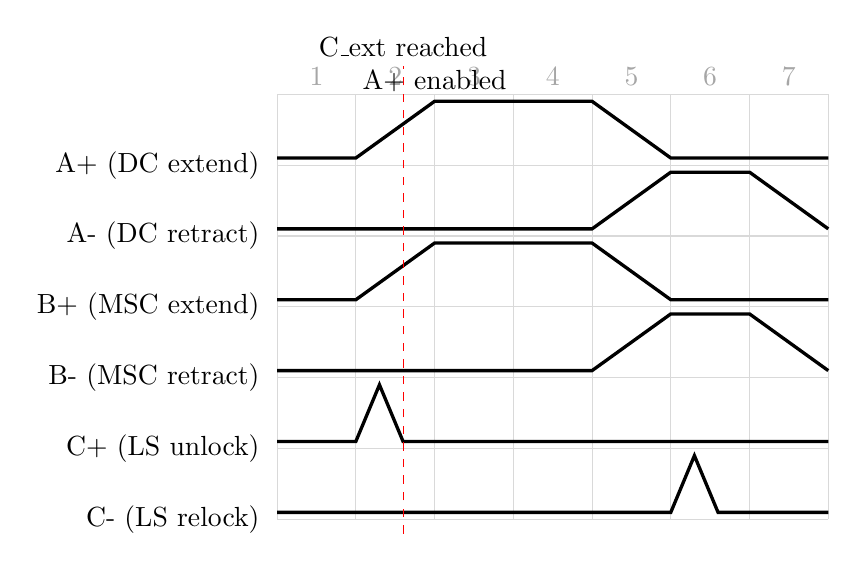
\begin{tikzpicture}[x=1cm,y=0.9cm]
	% grid and guides
	\draw[gray!30] (0,0) grid[xstep=1,ystep=1] (7,6);
	% step labels
	\foreach \s in {1,...,7} \node[gray!70] at (\s-0.5,6.25) {\s};
	% signal labels on the left
	\node[left] at (-0.1,5) {A+ (DC extend)};
	\node[left] at (-0.1,4) {A- (DC retract)};
	\node[left] at (-0.1,3) {B+ (MSC extend)};
	\node[left] at (-0.1,2) {B- (MSC retract)};
	\node[left] at (-0.1,1) {C+ (LS unlock)};
	\node[left] at (-0.1,0) {C- (LS relock)};

	% helper: low ~ +0.1, high ~ +0.9 within each lane
	% A+ (extend doors during opening: steps 2->3, hold until 4 then off)
	\draw[very thick] (0,5.1) -- (1,5.1) -- (2,5.9) -- (4,5.9) -- (5,5.1) -- (7,5.1);
	% A- (retract doors during closing: 4->6 window)
	\draw[very thick] (0,4.1) -- (4,4.1) -- (5,4.9) -- (6,4.9) -- (7,4.1);
	% B+ (extend metro slider with doors opening: 2->4)
	\draw[very thick] (0,3.1) -- (1,3.1) -- (2,3.9) -- (4,3.9) -- (5,3.1) -- (7,3.1);
	% B- (retract metro slider with doors closing: 4->6)
	\draw[very thick] (0,2.1) -- (4,2.1) -- (5,2.9) -- (6,2.9) -- (7,2.1);
	% C+ (unlock pulse around step 1)
	\draw[very thick] (0,1.1) -- (1,1.1) -- (1.3,1.9) -- (1.6,1.1) -- (7,1.1);
	% C- (relock confirm pulse near step 5)
	\draw[very thick] (0,0.1) -- (5,0.1) -- (5.3,0.9) -- (5.6,0.1) -- (7,0.1);

	% Interlock annotation: A+ only after C reaches max extension
	\draw[dashed,red] (1.6,-0.2) -- (1.6,6.4) node[above,black] {C\_ext reached};
	\node[above] at (2,5.9) {A+ enabled};
\end{tikzpicture}
\caption{Pneumatic position diagram (normal): A+/B+ during opening, A-/B- during closing. Interlock: A+ rises only after C is fully extended (C\_ext).}
\end{figure}

	\textbf{NOTE:} The time diagram above mirrors the tabular sequence.

% Obstruction/human-detected variant (IR or proximity sensor)
\begin{figure}[h]
\centering
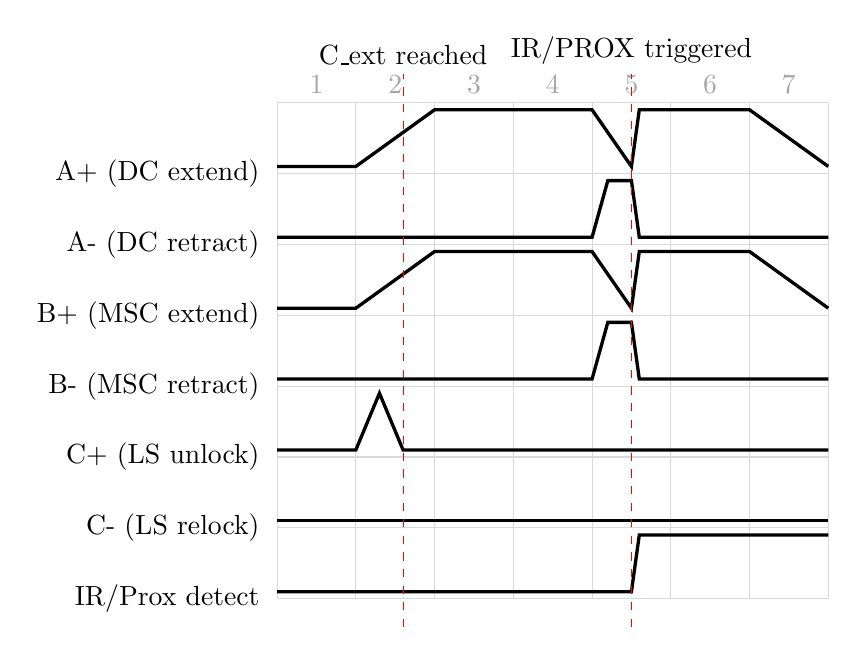
\begin{tikzpicture}[x=1cm,y=0.9cm]
	% grid and guides
	\draw[gray!30] (0,0) grid[xstep=1,ystep=1] (7,7);
	% step labels
	\foreach \s in {1,...,7} \node[gray!70] at (\s-0.5,7.25) {\s};
	% signal labels on the left
	\node[left] at (-0.1,6) {A+ (DC extend)};
	\node[left] at (-0.1,5) {A- (DC retract)};
	\node[left] at (-0.1,4) {B+ (MSC extend)};
	\node[left] at (-0.1,3) {B- (MSC retract)};
	\node[left] at (-0.1,2) {C+ (LS unlock)};
	\node[left] at (-0.1,1) {C- (LS relock)};
	\node[left] at (-0.1,0) {IR/Prox detect};

	% helper: low ~ +0.1, high ~ +0.9 within each lane
	% Choose obstruction time around mid-closing (e.g., x=4.5)
	% A+ normal open (2->4), then obstruction triggers immediate re-open (4.5->6)
	\draw[very thick] (0,6.1) -- (1,6.1) -- (2,6.9) -- (4,6.9)
					  -- (4.5,6.1) -- (4.5,6.1) -- (4.6,6.9) -- (6,6.9) -- (7,6.1);
	% A- starts closing at 4 but is aborted at 4.5
	\draw[very thick] (0,5.1) -- (4,5.1) -- (4.2,5.9) -- (4.5,5.9) -- (4.6,5.1) -- (7,5.1);
	% B+ normal open (2->4), then re-open after obstruction (4.5->6)
	\draw[very thick] (0,4.1) -- (1,4.1) -- (2,4.9) -- (4,4.9)
					  -- (4.5,4.1) -- (4.6,4.9) -- (6,4.9) -- (7,4.1);
	% B- starts at 4 but is aborted at 4.5
	\draw[very thick] (0,3.1) -- (4,3.1) -- (4.2,3.9) -- (4.5,3.9) -- (4.6,3.1) -- (7,3.1);
	% C+ as before (unlock pulse around 1)
	\draw[very thick] (0,2.1) -- (1,2.1) -- (1.3,2.9) -- (1.6,2.1) -- (7,2.1);
	% C- relock is inhibited due to obstruction (remains low)
	\draw[very thick] (0,1.1) -- (7,1.1);
	% IR/Prox detection goes high at obstruction time (4.5)
	\draw[very thick] (0,0.1) -- (4.5,0.1) -- (4.6,0.9) -- (7,0.9);

	% Event markers
	\draw[dashed,red] (4.5,-0.4) -- (4.5,7.4) node[above,black] {IR/PROX triggered};
	\draw[dashed,red] (1.6,-0.4) -- (1.6,7.4) node[above,black] {C\_ext reached};
\end{tikzpicture}
\caption{Obstruction/human-detected variant: IR/Prox trigger during closing causes immediate re-open (A+/B+ high again) and inhibits relock (C- stays low). A+ remains interlocked to C\_ext for any new opening.}
\end{figure}

% =============================================================
\section{Milestone Deliverables Checklist}
\begin{itemize}[noitemsep]
	\item Updated project description (single-cylinder dual-rack architecture) -- \textit{Revised}
	\item 3D views of mechanical design -- \textit{Cover render inserted; exploded view pending}
	\item Mechanical component list -- \textit{Reworked for 3 actuators}
	\item DFM report + 2D drawings -- \textit{Framework ready; drawings pending}
	\item DFA report with exploded views -- \textit{Framework ready; views pending}
	\item Pneumatic position-step diagram -- \textit{Updated table; graphic pending}
	\item Sensor + safety logic (IR + reed) -- \textit{Documented}
	\item Mechanism and lock figures -- \textit{Inserted}
	\item SolidWorks 3D design files -- \textit{To include in ZIP upon completion}
\end{itemize}

% =============================================================
\section{Appendix}
\subsection*{A. Datasheets}
	\textbf{NOTE:} Insert PDFs (referenced externally) or summary tables for each purchased component.\\
\fbox{\parbox{0.9\linewidth}{Datasheet Collection Placeholder -- TODO}}
\subsection*{B. Engineering Calculations}
	\textbf{NOTE:} Force sizing for cylinders, friction coefficients, air consumption estimates.\\
\fbox{\parbox{0.9\linewidth}{Calculation Sheets Placeholder -- TODO}}
\subsection*{C. Risk and Safety Notes}
Preliminary safety considerations: pinch points at door edges, emergency stop circuit design, pneumatic pressure limits. Detailed FMEA optional in later milestone.\\
	\textbf{NOTE:} Insert safety assessment here.

\end{document}
